% The same study written as an ordinary LaTeX manuscript, the way it would be sent to a journal.
% It compiles with pdflatex + bibtex, and HyperTeX opens it as is (compatibility mode):
% \input files, the PDF figure, \cref and the BibTeX bibliography (paper.bbl) all work.
\documentclass[11pt]{article}
\usepackage{amsmath,amssymb}
\usepackage{graphicx}
\usepackage{hyperref}
\usepackage{cleveref}

\newcommand{\dd}{\mathrm{d}}
\newcommand{\wn}{\omega_0}
\newcommand{\abs}[1]{\left\lvert #1 \right\rvert}
\newtheorem{proposition}{Proposition}

\title{Resonance in a Damped, Driven Oscillator}
\author{krunyx \and HyperTeX examples}
\date{November 2026}

\begin{document}
\maketitle

\begin{abstract}
We derive the steady response of a linear oscillator with viscous damping to a harmonic force and
compare the predicted resonance curve with a simulated air-track experiment. This manuscript is the
LaTeX twin of the HyperTeX report
\href{https://krunyx.com/examples/oscillator/report.htex}{report.htex}, which adds live sliders.
\end{abstract}

\section{Introduction}\label{sec:intro}
Resonance appears whenever a system with a natural frequency is driven periodically: in mechanical
structures, electrical circuits and the absorption of light by atoms~\cite{French1971}. The
simplest model is a mass on a spring with viscous friction, treated in every mechanics
text~\cite{Taylor2005,Landau1976}. \Cref{sec:model} sets up the model and \cref{sec:resonance}
derives the resonance curve shown in \cref{fig:resonance}.

\section{Model}\label{sec:model}
A mass $m$ attached to a spring of stiffness $k$ and a damper with coefficient $c$, driven by
$F_0\cos\Omega t$, obeys
\begin{equation}\label{eq:motion}
  m\ddot x + c\dot x + kx = F_0\cos\Omega t .
\end{equation}
With $\wn = \sqrt{k/m}$ and $\zeta = c/(2\sqrt{mk})$ this becomes
\begin{equation}\label{eq:normal}
  \ddot x + 2\zeta\wn\dot x + \wn^2 x = \frac{F_0}{m}\cos\Omega t .
\end{equation}
For $\zeta<1$ the free solution decays as $e^{-\zeta\wn t}$ while oscillating at
$\omega_\mathrm{d} = \wn\sqrt{1-\zeta^2}$.

\section{Steady response}\label{sec:resonance}
Substituting $x = \operatorname{Re}\bigl(\hat x\,e^{i\Omega t}\bigr)$ into \cref{eq:normal} and
writing $r = \Omega/\wn$ gives
\begin{equation}\label{eq:amp}
  \frac{\abs{\hat x}}{F_0/k} = \frac{1}{\sqrt{(1-r^2)^2 + (2\zeta r)^2}} .
\end{equation}

\begin{proposition}\label{prop:peak}
For $\zeta < 1/\sqrt{2}$ the amplitude~\eqref{eq:amp} peaks at $r = \sqrt{1-2\zeta^2}$ with height
$1/\bigl(2\zeta\sqrt{1-\zeta^2}\bigr)$.
\end{proposition}

\begin{figure}[ht]
  \centering
  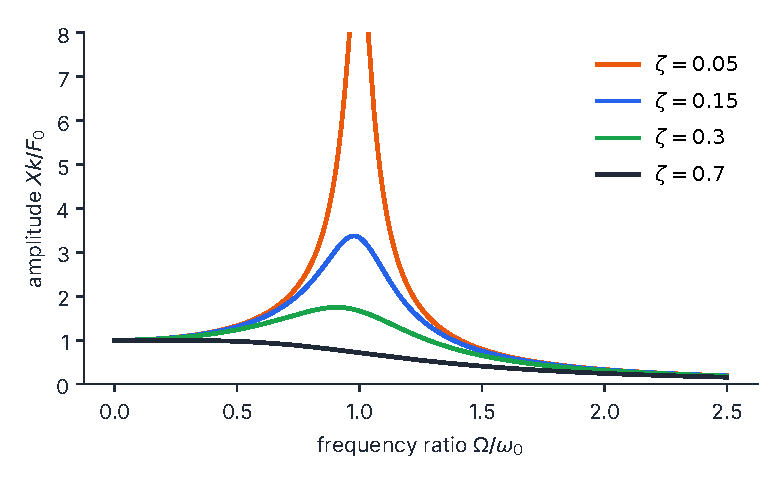
\includegraphics[width=0.75\linewidth]{figures/resonance.pdf}
  \caption{Resonance curves~\eqref{eq:amp} for four damping ratios.}
  \label{fig:resonance}
\end{figure}

\begin{table}[ht]
  \centering
  \caption{Fitted parameters (simulated data).}\label{tab:fit}
  \begin{tabular}{lrr}
    \hline
    Quantity & Value & Uncertainty \\
    \hline
    $\wn/2\pi$ & 1.62 Hz & 0.01 Hz \\
    $\zeta$ & 0.061 & 0.004 \\
    $Q = 1/(2\zeta)$ & 8.2 & 0.5 \\
    \hline
  \end{tabular}
\end{table}

The fitted values in \cref{tab:fit} give a peak height of $8.2$, in line with
\cref{prop:peak}. A quality factor this large means the oscillator selects a narrow band of
frequencies~\cite{Landau1976}.


\bibliographystyle{plain}
\bibliography{refs}
\end{document}
